% ---------
%  Compile with "pdflatex hw0".
% --------
%!TEX TS-program = pdflatex
%!TEX encoding = UTF-8 Unicode

\documentclass[11pt]{article}
\usepackage{jeffe,handout,graphicx}
\usepackage[utf8]{inputenc}		% Allow some non-ASCII Unicode in source
\usepackage[dvipsnames]{xcolor}
\usepackage{mdframed}
\usepackage{arydshln}

\setlength{\dashlinedash}{0.2pt}
\setlength{\dashlinegap}{1.5pt}

\headers{CS 6363.003}{Homework 3 (due April 4)}{Spring 2021}

% =========================================================
\begin{document}

\title{CS 6363.003 Homework 3}
\author{Due Sunday April 4th on eLearning}
\date{March 20, 2021}

\maketitle

Please answer the following \EMPH{\(4\)} questions, some of which have multiple parts.

% ---------------------------------------------------------

\begin{problems}
\item
  Suppose you are given a sequence of integers separated by \(+\) and \(-\) signs;
  for example:
  \[ 1 + 3 - 2 - 5 + 1 - 6 + 7 \]

  You can change the value of this expression by adding parentheses in different places.
  For example:
  \[ 1 + 3 - 2 - 5 + 1 - 6 + 7 = -1 \]
  \[ (1 + 3 - (2 - 5)) + (1 - 6) + 7 = 9 \]
  \[ (1 + (3 - 2)) - (5 + 1) - (6 + 7) = -17 \]

  Describe and analyze a dynamic programming algorithm to compute, given a list of integers
  separated by \(+\) and \(-\) signs, the maximum possible value the expression can take by adding
  parentheses.
  Parentheses must be used only to group additions and subtractions;
  in particular, \emph{do not} use them to create implicit multiplication as in \(1 + 3(-2)(-5) + 1
  - 6 + 7 = 33\).
  
  \paragraph*{Clarification} 
  The unary \(-\) operators one would normally use to denote negative integers are not included in
  the collection of \(+\) and \(-\) signs separating the integers of the input sequence.
  For example, suppose one is given the following sequence of integers separated by \(+\) and \(-\)
  signs:
  \[ 3 + (-2) - 6 - (-4)  \]

  The \((-2)\) and the \((-4)\) are to be treated as a \(-2\) and \(-4\), respectively, in any
  method of adding parentheses considered by the algorithm.
  In particular, there are exactly five distinct ways to group the \(+\) and \(-\) operations in
  this sequence using parentheses (some of which evaluate to the same result):
  
  \[ 3 + ((-2) - (6 - (-4))) = 15 \]
  \[ 3 + (((-2) - 6) - (-4)) = -1 \]
  \[ (3 + (-2)) - (6 - (-4)) = -9 \]
  \[ (3 + ((-2) - 6)) - (-4) = -1 \]
  \[ ((3 + (-2)) - 6) - (-4) = -1 \]

\item
  Let~\(T\) be a rooted binary tree with~\(n\) vertices, and let~\(k \leq n\) be a positive integer.
  We would like to mark~\(k\) vertices in~\(T\) so that every vertex has a nearby marked ancestor.
  More formally, we define the \EMPH{clustering cost} of any subset~\(K\) of vertices as
  \[ cost(K) = \max_{v} cost(v, K), \]
  where the maximum is taken over all vertices~\(v\) in the tree, and \(cost(v, K)\) is the distance
  from~\(v\) to its nearest ancestor in~\(K\):
  \[ cost(v, K) =
    \begin{cases}
      0 &\text{ if \(v \in K\)}\\
      \infty &\text{ if \(v\) is the root of \(T\) and \(v \notin K\)}\\
      1 + cost(parent(v)) &\text{ otherwise}
    \end{cases}
  \]

  In particular, \(cost(K) = \infty\) if \(K\) excludes the root of~\(T\).
  \begin{figure}[h]
    \centering
    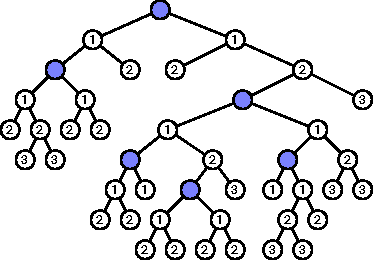
\includegraphics{figs/clustering_cost}
    \label{fig:clustering_cost}
    \caption{A subset of six vertices in a binary tree with clustering cost~\(3\).
    The other vertices are labeled with the distance to their nearest ancestor in the subset.}
  \end{figure}

  \begin{enumerate}
    \item
      Describe a dynamic programming algorithm to compute, given the tree~\(T\) and an
      integer~\(r\), the size of the smallest subset of vertices whose clustering cost is at
      most~\(r\).
      For full credit, your algorithm should run in~\(O(nr)\) time.

    \item
      Describe an algorithm to compute, given the tree~\(T\) and an integer~\(k\), the minimum
      clustering cost of any subset of~\(k\) vertices in~\(T\).
      For full credit, your algorithm should run in~\(O(n^2 \log n)\) time.
      \emph{[Hint: Use your algorithm for part (a) as a subroutine.
      You may assume your algorithm for part (a) is correct and runs in~\(O(nr)\) time.]}
  \end{enumerate}

\item
  Describe and analyze an algorithm to compute an optimal \emph{ternary} prefix-free code for a
  given array of frequencies~\(f[1~..~n]\).
  In other words, each character in the alphabet should be assigned a string of \(0\)s, \(1\)s, and
  \(2\)s such that no code is a prefix of any other and the total length of the encoded message
  represented by the frequencies is as small as possible.
  Similar to what we saw in lecture, your output can be the representation of a ternary code tree.
  See Figure 4.4 of Erickson 4 and the preceding text for an example of how to build an optimal
  \emph{binary} code tree.

  For simplicity, you may consider the empty string to be a valid code word for the case \(n = 1\).
  Don't forget to prove that your algorithm is correct for \emph{all} \(n\).

\item
  There are \(n\) galaxies connected by \(m\) intergalactic teleport-ways.
  Each teleport-way joins two galaxies and can be traversed in both directions.
  Also, each teleport-way~\(e\) has an associated cost~\(c(e)\) of dollars, where~\(c(e)\) is a
  positive integer.
  A teleport-way can be used multiple times, but the toll must be paid every time it is used.

  Judy wants to travel from galaxy~\(s\) to galaxy~\(t\), but teleportation is not very pleasant and
  she would like to minimize the number of times she needs to teleport.
  However, she wants the total cost to be a multiple of five dollars, because carrying small change
  is not pleasant either.

  Describe and analyze an algorithm to compute the smallest number of times Judy needs to teleport
  to travel from galaxy~\(s\) to galaxy~\(t\) so that the total cost is a multiple of five dollars.
  To emphasize, Judy wants to minimize the \emph{number of times she teleports}.
  Any total cost is fine as long as it is a multiple of five dollars.
  
  \emph{[Hint: Build a graph that can model Judy's location and how much small change she has.
  Then, run an appropriate graph search algorithm that you've seen before.]}
\end{problems}
\end{document}
